\documentclass[10pt]{book}
\usepackage[sectionbib]{natbib}
\usepackage{array,epsfig,fancyheadings,rotating,caption}
\usepackage{hyperref}
\usepackage{mycommands}
%%%%%%%%%%%%%%%%%%%%%%%%%%%%%%%%%%%%%%%%%%%%%%%%%%%%%%%%%%%%%%%%%%%%%%%%%%%%%%%%%%%%%%%%%%%%%%%%%%%%%%%%%%%%%%%%%%%%%%%%%%%%

\textwidth=31.9pc
\textheight=46.5pc
\oddsidemargin=1pc
\evensidemargin=1pc
\headsep=15pt
%\headheight=.2cm
\topmargin=.6cm
\parindent=1.7pc
\parskip=0pt

\usepackage{amsmath}
\usepackage{amssymb}
\usepackage{amsfonts}
\usepackage{multirow}
\usepackage{amsthm}

\setcounter{page}{1}
\pagestyle{fancy}

%%%%%%%%%%%%%%%%%%%%%%%%%%%%%%%%%%%%%%%%%%%%%%%%%%%%%%%%%%%%%%%%%%%%%%%%%%%%%%%%%%%%%%%%%%%%%%%%%%%%%%%%%%%%%%%%%%%%%%%%%%%%
\pagestyle{fancy}
\def\n{\noindent}
\lhead[\fancyplain{} \leftmark]{}
\chead[]{}
\rhead[]{\fancyplain{}\rightmark}
\cfoot{}

%%%%%%%%%%%%%%%%%%%%%%%%%%%%%%%%%%%%%%%%%%%%%%%%%%%%%%%%%%%%%%%%%%%%%%%%%%%%%%%%%%%%%%%%%%%%%%%%%%%%%%%%%%%%%%%%%%%%%%%%%%%%
%%%%%%%%%%%%%%%%%%%%%%%%%%%%%%%%%%%%%%%%%%%%%%%%%%%%%%%%%%%%%%%%%%%%%%%%%%%%%%%%%%%%%%%%%%%%%%%%%%%%%%%%%%%%%%%%%%%%%%%%%%%%

\begin{document}

\newtheorem{Theorem}{Theorem}[section]
\newtheorem{Lemma}[Theorem]{Lemma}
\newtheorem{Corollary}[Theorem]{Corollary}
\theoremstyle{definition} \newtheorem{Definition}[Theorem]{Definition}
%\newtheorem{proof}{Proof}
\newtheorem{example}{Example}
\newtheorem{remark}{Remark}

%%%%%%%%%%%%%%%%%%%%%%%%%%%%%%%%%%%%%%%%%%%%%%%%%%%%%%%%%%%%%%%%%%%%%%%%%%%%%%%%%%%%%%%%%%%%%%%%%%%%%%%%%%%%%%%%%%%%%%%%%%%%
%%%%%%%%%%%%%%%%%%%%%%%%%%%%%%%%%%%%%%%%%%%%%%%%%%%%%%%%%%%%%%%%%%%%%%%%%%%%%%%%%%%%%%%%%%%%%%%%%%%%%%%%%%%%%%%%%%%%%%%%%%%%

%\renewcommand{\baselinestretch}{1.2}

\markright{ \hbox{\footnotesize\rm Statistica Sinica
%{\footnotesize\bf 24} (201?), 000-000
}\hfill\\[-13pt]
\hbox{\footnotesize\rm
%\href{http://dx.doi.org/10.5705/ss.20??.???}{doi:http://dx.doi.org/10.5705/ss.20??.???}
}\hfill }

\markboth{\hfill{\footnotesize\rm FIRSTNAME1 LASTNAME1 AND FIRSTNAME2 LASTNAME2} \hfill}
{\hfill {\footnotesize\rm FILL IN A SHORT RUNNING TITLE} \hfill}

\renewcommand{\thefootnote}{}
$\ $\par

%%%%%%%%%%%%%%%%%%%%%%%%%%%%%%%%%%%%%%%%%%%%%%%%%%%%%%%%%%%%%%%%%%%%%%%%%%%%%%%%%%%%%%%%%%%%%%%%%%%%%%%%%%%%%%%%%%%%%%%%%%%%

\fontsize{10.95}{14pt plus.8pt minus .6pt}\selectfont
\vspace{0.8pc}
\centerline{\large\bf Robust estimation of principal components}
\vspace{2pt}
\centerline{\large\bf from depth-based multivariate rank covariance matrix}
\vspace{.4cm}
\centerline{Author(s)}
\vspace{.4cm}
\centerline{\it Affiliation(s)}
\vspace{.55cm}
\fontsize{9}{11.5pt plus.8pt minus .6pt}\selectfont

%%%%%%%%%%%%%%%%%%%%%%%%%%%%%%%%%%%%%%%%%%%%%%%%%%%%%%%%%%%%%%%%%%%%%%%%%%%%%%%%%%%%%%%%%%%%%%%%%%%%%%%%%%%%%%%%%%%%%%%%%%%%

\begin{quotation}
\noindent {\it Abstract:}
Analyzing principal components for multivariate data from its spatial sign covariance matrix (SCM) has been proposed as a computationally simple and robust alternative to normal PCA, but it suffers from poor efficiency properties and is actually inadmissible with respect to the maximum likelihood estimator. Here we use data depth-based spatial ranks in place of spatial signs to obtain the orthogonally equivariant Depth Covariance Matrix (DCM) and use its eigenvector estimates for PCA. We derive asymptotic properties of the sample DCM and influence functions of its eigenvectors. The shapes of these influence functions indicate robustness of estimated principal components, and good efficiency properties compared to the SCM. Finite sample simulation studies show that principal components of the sample DCM are robust with respect to deviations from normality, as well as are more efficient than the SCM and its affine equivariant version, Tyler's shape matrix. Through two real data examples, we also show the effectiveness of DCM-based PCA in analyzing high-dimensional data and outlier detection, and compare it with other methods of robust PCA.
\par

\vspace{9pt}
\noindent {\it Key words and phrases:}
Data depth; Principal components analysis; Robustness; Sign covariance matrix; Multivariate ranking
\par
\end{quotation}\par

\def\thefigure{\arabic{figure}}
\def\thetable{\arabic{table}}

\fontsize{10.95}{14pt plus.8pt minus .6pt}\selectfont

\setcounter{chapter}{1}
\setcounter{equation}{0} %-1
\noindent {\bf 1. Introduction}

In multivariate analysis, the study of principal components is important since it provides a small number of uncorrelated variables from a potentially larger number of variables, so that these new components explain most of the underlying variability in the original data. In case of multivariate normal distribution, the sample covariance matrix provides the most asymptotically efficient estimates of eigenvectors/ principal components, but it is extremely sensitive to outliers as well as relaxations of the normality assumption. To address this issue, several robust estimators of the population covariance or correlation matrix have been proposed which can be used for Principal Components Analysis (PCA). They can be roughly put into these categories: robust, high breakdown point estimators that are computation-intensive \citep{rousseeuw85, maronna76}; M-estimators that are calculated by simple iterative algorithms but do not necessarily possess high breakdown point \citep{huber77, tyler87}; and symmetrised estomators that are highly efficient and robust to deviations from normality, but sensitive to outliers and computationally demanding \citep{dumbgen98, sirkia07}.

When principal components are of interest, one can also estimate the population eigenvectors by analyzing the spatial sign of a multivariate vector: the vector divided by its magnitude, instead of the original data. The covariance matrix of these sign vectors, namely Sign Covariance Matrix (SCM) has the same set of eigenvectors as the covariance matrix of the original population, thus the multivariate sign transformation yields computationally simple and high-breakdown estimates of principal components \citep{locantore99, visuri00}. Although the SCM is not affine equivariant, its orthogonal equivariance suffices for the purpose of PCA. However, the resulting estimates are not very efficient, and are in fact asymptotically inadmissible \citep{magyar14}, in the sense that there is an estimator (Tyler's M-estimate of scatter, to be precise) that has uniformly lower asymptotic risk than the SCM.

The nonparametric concept of data-depth had first been proposed by \cite{tukey75} when he introduced the halfspace depth. Given a dataset, the depth of a given point in the sample space measures how far inside the data cloud the point exists. An overview of statistical depth functions can be found in \citep{zuo00}. Depth-based methods have recently been popular for robust nonparametric classification \citep{jornsten04, ghosh05, dutta12, sguera14}. In parametric estimation, depth-weighted means \citep{ZuoCuiHe04} and covariance matrices \citep{ZuoCui05} provide high-breakdown point as well as efficient estimators, although they do involve choice of a suitable weight function and tuning parameters. In this paper we study the covariance matrix of the multivariate rank vector that is obtained from the data-depth of a point and its spatial sign, paying special attention to its eigenvectors. Specifically, we develop a robust version of principal components analysis for elliptically symmetric distributions based on the eigenvectors of this covariance matrix, and compare it with normal PCA and spherical PCA, i.e. PCA based on eigenvectors of the SCM.

The paper is arranged in the following fashion. Section 2 provides preliminary theoretical concepts required for developments in the subsequent sections. Section 3 introduces the Depth Covariance Matrix (DCM) and states some basic results related to this. Section 4 provides asymptotic results regarding the sample DCM, calculated using data depths with respect to the empirical distribution function, as well as its eigenvectors and eigenvalues. Section 5 focuses solely on principal component estimation using the sample DCM. We obtain influence functions and asymptotic efficiencies for eigenvectors of the DCM. We also compare their finite sample efficiencies for several multinormal and multivariate $t$-distributions with those of the SCM, Tyler's scatter matrix and its depth-weighted version through a simulation study. Section 6 presents two applications of the methods we develop on real data. Finally, we wrap up our discussion in Section 7 by giving a summary of our findings and providing some potential future areas of research. Proofs of all the results we derive are given in the appendix.
\par

\vspace{1em}
\setcounter{chapter}{2}
\setcounter{equation}{0} %-1
\noindent {\bf 2. Preliminaries}

Given a vector $\bfx \in \mathbb{R}^p$, its spatial sign is defined as the vector valued function \citep{locantore99}:
%
$$ \bfS(\bfx) = \begin{cases} \bfx\| \bfx \|^{-1} \quad \mbox{if }\bfx \neq \bf0\\
\bf0 \quad \mbox{if }\bfx = \bf0 \end{cases} $$
%
When $\bfx$ is a random vector that follows an elliptic distribution $|\Sigma|^{-1/2} f((\bfx - \bfmu)^T \Sigma^{-1} (\bfx - \bfmu))$, with a mean vector $\bfmu$ and covariance matrix $\Sigma$, the sign vectors $\bfS(\bfx - \bfmu)$ reside on the surface of a $p$-dimensional unit ball centered at $\bfmu$. Denote by $\Sigma_S(\bfX) = E\bfS (\bfX - \bfmu)\bfS (\bfX - \bfmu)^T$ the covariance matrix of spatial signs, or the \textit{Sign Covariance Matrix} (SCM). The transformation $\bfx \mapsto \bfS(\bfx - \bfmu)$ keeps eigenvectors of population covariance matrix unchanged, and eigenvectors of the sample SCM $ \hat \Sigma_S = \sum_{i=1}^n \bfS (\bfx_i - \bfmu)\bfS (\bfx_i - \bfmu)^T/n $ are $\sqrt n$-consistent estimators of their population counterparts \citep{taskinen12}.

The sign transformation is rotation equivariant, i.e. $ \bfS(P (\bfx - \bfmu)) = P(\bfx - \bfmu)/\| P (\bfx - \bfmu)\| = P(\bfx - \bfmu)/\|\bfx - \bfmu\| = P \bfS(\bfx - \bfmu)$ for any orthogonal matrix $P$, and as a result the SCM is rotation equivariant too, in the sense that $\Sigma_S(P\bfX) = P \Sigma_S(\bfX) P^T$. This is not necessarily true in general if $P$ is replaced by any non-singular matrix. An affine equivariant version of the sample SCM is obtained as the solution $\hat \Sigma_T$ of the following equation:
%
$$ \hat \Sigma_T(\bfX) = \frac{p}{n} \sum_{i=1}^n \frac{(\bfx - \bfmu)(\bfx - \bfmu)^T}{(\bfx - \bfmu)^T \hat\Sigma_T(\bfX)^{-1} (\bfx - \bfmu)} $$
%
which turns out to be Tyler's M-estimator of scatter \citep{tyler87}. In this context, one should note that for scatter matrices, affine equivariance will mean any affine transformation on the original random variable $\bfX \mapsto \bfX^* = A\bfX + \bfb$ ($A$ non-singular, $\bfb \in \mathbb{R}^p$) being carried over to the covariance matrix estimate upto a scalar multiple: $\hat\Sigma_T(\bfX^*) = k. A \hat\Sigma_T(\bfX) A^T$ for some $k>0$.

\vspace{.5em}
\noindent {\bf 2.1 Data depth and outlyingness}

For any multivariate distribution $F = F_\bfX$, the depth of a point $\bfx \in \mathbb{R}^p$, say $D(\bfx, F_\bfX)$ is any real-valued function that provides a 'center outward ordering' of $\bfx$ with respect to $F$ \citep{zuo00}. \cite{liu90} outlines the desirable properties of a statistical depth function:

\noindent
(P1) Affine invariance: $D(A\bfx + \bfb, F_{A\bfX+\bfb}) = D(\bfx, F_\bfX)$\\
(P2) Maximality at center: $D(\bftheta, F_\bfX) = \sup_{\bfx\in \mathbb{R}^p} D(\bfx, F_\bfX)$ for $F_\bfX$ having center of symmetry $\bftheta$. This point is called the \textit{deepest point} of the distribution.\\
(P3) Monotonicity with respect to deepest point: $D(\bfx; F_\bfX) \leq D(\bftheta + a(\bfx - \bftheta), F_\bfX)$, $\bftheta$ being deepest point of $F_\bfX$.\\
(P4) Vanishing at infinity: $D(\bfx; F_\bfX) \rightarrow \bf0$ as $\|\bfx\| \rightarrow \infty $.

In (P2) the types of symmetry considered can be central symmetry, angular symmetry and halfspace symmetry. Also for multimodal probability distributions, i.e. distributions with multiple local maxima in their probability density functions, properties (P2) and (P3) are actually restrictive towards the formulation of a reasonable depth function that captures the shape of the data cloud. In our derivations that follow, we replace these two by a slightly weaker condition: (P2*) The \textit{existence} of a maximal point, i.e. $ \sup_{\bfx\in \mathbb{R}^p} D(\bfx, F_\bfX) < \infty $. We denote this point by $M_D(F)$.

A real-valued function measuring the outlyingness of a point with respect to the data cloud can be seen as the opposite of what data depth does. Indeed, such functions have been used to define several depth functions, for example simplicial volume depth, projection depth and $L_p$-depth. Here we give a general definition of such functions as a transformation on any depth function:

\begin{Definition}
Given a random variable $\bfX$ following a probability distribution $F$, and a depth function $D(.,.)$, we define Htped of a point $\bfx$ as: $\tilde D(\bfx, F) = h(d_\bfx)$ as any function of the data depth $D(\bfx, F) = d_\bfx$ so that $h(d_\bfx)$ is bounded, monotonically decreasing in $d_\bfx$ and $\sup_\bfx \tilde D(\bfx, F) < \infty$.
\end{Definition}

For a fixed depth function, there are several choices of a corresponding htped. We develop our theory assuming a general htped function, but for the plots and simulations, fix our htped as $\tilde D(\bfx, F) = M_D(F) - D(\bfx, F)$, i.e. simply subtract the depth of a point from the maximum possible depth over all points in sample space.

We will be using the following 3 measures of data-depth to obtain our DCMs and compare their performances:

\begin{itemize}
\item \textbf{Halfspace depth} (HD) \citep{tukey75} is defined as the minimum probability of all halfspaces containing a point. In our notations,

$$ HD(\bfx, F)  = \inf_{\bfu \in \mathbb{R}^p; \bfu \neq \bf0} P(\bfu^T \bfX \geq \bfu^T \bfx) $$

\item \textbf{Mahalanobis depth} (MhD) \citep{LiuPareliusSingh99} is based on the Mahalanobis distance of $\bfx$ to $\bfmu$ with respect to $\Sigma$: $d_\Sigma(\bfx, \bfmu) = \sqrt{(\bfx - \bfmu)^T \Sigma^{-1} (\bfx - \bfmu)}$. It is defined as

$$ MhD(\bfX, F) = \frac{1}{1 + d^2_\Sigma (\bfx - \bfmu)} $$

note here that $d_\Sigma(\bfx,\bfmu)$ can be seen as a valid htped function of $\bfx$ with respect to $F$.

\item \textbf{Projection depth} (PD) \citep{zuo03} is another depth function based on an outlyingness function. Here that function is

$$ O(\bfx, F) = \sup_{\| \bfu \| = 1} \frac{| \bfu^T\bfx - m(\bfu^T\bfX)|}{s(\bfu^T\bfX)} $$

where $m$ and $s$ are some univariate measures location and scale, respectively. Given this the depth at $\bfx$ is defined as $PD(\bfx, F) = 1/(1+O(\bfx, F))$.
\end{itemize}

Computation-wise, MhD is easy to calculate since the sample mean and covariance matrix are generally used as estimates of $\mu$ and $\Sigma$, respectively. However this makes MhD less robust with respect to outliers. PD is generally approximated by taking maximum over a number of random projections. There have been several approaches for calculating HD. A recent unpublished paper \citep{rainerArxiv} provides a general algorithm that computes exact HD in $O(n^{p-1}\log n)$ time. In this paper, we shall use inbuilt functions in the R package \texttt{fda.usc} for calculating the above depth functions.

\vspace{1em}
\setcounter{chapter}{3}
\setcounter{equation}{0} %-1
\noindent {\bf 3. Depth-based rank covariance matrix}\vspace{1em}

Consider a vector-valued random variable $\bfX \in \mathbb{R}^p$. Data depth is as much a property of the random variable as it is of the underlying distribution, so for ease of notation while working with transformed random variables, from now on we shall be using $D_\bfX(\bfx) = D(\bfx, F)$ to denote the depth of a point $\bfx$. Now, given a depth function $D_{\bfX}(\bfx)$ (equivalently, an htped function $\tilde D_\bfX(\bfx) = \tilde D(\bfx, F)$), transform the original random variable as: $\tilde \bfx = \tilde D_\bfX(\bfx) \bfS(\bfx - \bfmu)$, $\bfS(.)$ being the spatial sign functional. The transformed random variable $\tilde \bfX$ can be seen as the multivariate rank corresponding to $\bfX$ (e.g. \cite{serfling2006}). Figure \ref{fig:rankplot} gives an idea of how $\tilde \bfX$ is distributed when $\bfX$ has a bivariate normal distribution. Compared to the spatial sign, which are distributed on the surface of $p$-dimensional unit ball centered at $\bfmu$, these spatial ranks have the same direction as original data and reside \textit{inside} the $p$-dimensional ball around $\bfmu$ that has radius $M_D(F)$ (which, for the case of halfspace depth, equals 0.5).

\begin{figure}[t]
	\captionsetup{singlelinecheck=off}
	\centering
		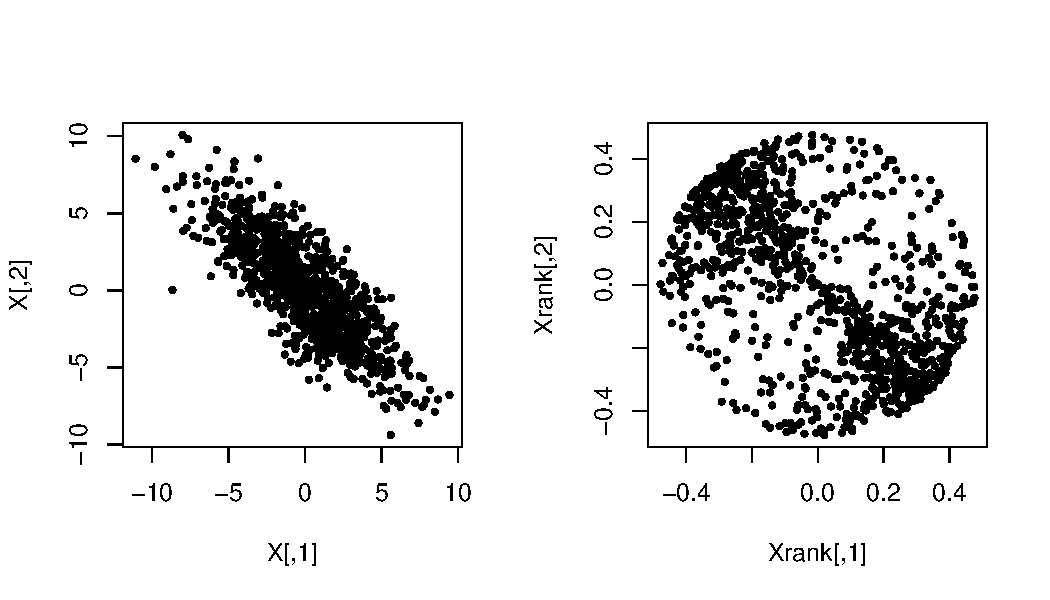
\includegraphics[height=6cm]{ranks}
	\caption{(Left) 1000 points randomly drawn from $\mathcal N_2\left((0,0)^T, \left(\protect\begin{smallmatrix} 5 & -4 \\ -4 & 5 \protect\end{smallmatrix}\right)\right) $ and (Right) their multivariate ranks based on halfspace depth}
	\label{fig:rankplot}
\end{figure}

Now consider the spectral decomposition for the covariance matrix of $F$: $\Sigma = \Gamma\Lambda\Gamma^T$, $\Gamma$ being orthogonal and $\Lambda$ diagonal with positive diagonal elements. Also normalize the original random variable as $\bfz = \Gamma^T\Lambda^{-1/2} (\bfx - \bfmu)$. In this setup, we can represent the transformed random variable as
%
\begin{eqnarray}
\tilde \bfx &=& \tilde D_{\bfX} (\bfx) \bfS(\bfX - \bfmu) \notag \\
&=& \tilde D_{\Gamma\Lambda^{1/2}\bfZ + \bfmu} (\Gamma\Lambda^{1/2} \bfz + \bfmu). \bfS(\Gamma\Lambda^{1/2} \bfz) \notag \\
&=& \Gamma \tilde D_{\bfZ}(\bfz) \bfS(\Lambda^{1/2}\bfz) \notag \\
&=& \Gamma \Lambda^{1/2} \tilde D_{\bfZ}(\bfz) \bfS(\bfz) \frac{\| \bfz \|}{\|\Lambda^{1/2} \bfz\|}
\label{equation:rankdecomp}
\end{eqnarray}
%
%Because of affine (thus rotational) invariance of a depth function, the depth (htped) value at $\bfz$ does not depend on the direction of $\bfz$, i.e. $\tilde D_{\bfZ}(\bfz)$ and $\bfS(\bfz)$ are independent. Furthermore,
%$$ Cov \left(\bfS (\bfz), \frac{\| \bfz \|}{\|\Lambda^{1/2} \bfz\|} \right) = E \left(\bfS (\bfz). \frac{\| \bfz \|}{\|\Lambda^{1/2} \bfz\|} \right) - E \bfS (\bfz) E \left(\frac{\| \bfz \|}{\|\Lambda^{1/2} \bfz\|} \right) = E \left( \frac{\bfz}{\|\Lambda^{1/2} \bfz\|} \right) = \bf0$$
%both $\bfS (\bfz)$ and $\bfz / \| \Lambda^{1/2}\bfz \|$ are odd functions of $\bfz$, which has a circularly symmetric distribution, hence each of them has expectation $\bf0$. Consequently, we obtain an expression for the covariance matrix of $\tilde \bfX$:

$\tilde D_\bfZ(\bfz)$ is an even function in $\bfz$ because of affine invariance, as is $\| \bfz \| / \|\Lambda^{1/2} \bfz \|$. Since $\bfS(\bfz)$ is odd in $\bfz$ for circularly symmetric $\bfz$, it follows that $E(\tilde \bfX) = \bf0$, and consequently we obtain an expression for the covariance matrix of $\tilde \bfX$:

\begin{Theorem} \label{Theorem:covform}
Let the random variable $\bfX \in \mathbb{R}^p$ follow an elliptical distribution with center $\bfmu$ and covariance matrix $\Sigma = \Gamma\Lambda\Gamma^T$, its spectral decomposition. Then, given a depth function $D_\bfX(.)$ the covariance matrix of the transformed random variable $\tilde\bfX$ is
\begin{equation} \label{equation:covformEq1}
Cov(\tilde \bfX) = \Gamma \Lambda_{D,S} \Gamma^T,\quad\mbox{with}\quad \Lambda_{D,S} = \mathbb E_\bfz \left[ (\tilde D_\bfZ(\bfz))^2 \frac{\Lambda^{1/2} \bfz \bfz^T \Lambda^{1/2}}{\bfz^T \Lambda \bfz} \right]
\end{equation}
where $\bfz = (z_1,...,z_p)^T \sim N({\bf 0}, I_p)$, so that $\Lambda_{D,S}$ a diagonal matrix with diagonal entries
%
$$ \lambda_{D,S,i} = \mathbb E_\bfZ \left[ \frac{(\tilde D_\bfZ(\bfz))^2 \lambda_i z_i^2}{\sum_{j=1}^p \lambda_j z_j^2} \right] $$
\end{Theorem}

The matrix of eigenvectors of the covariance matrix, $\Gamma$, remains unchanged in the transformation $\bfX \rightarrow \tilde \bfX$. As a result, the multivariate rank vectors can be used for robust principal component analysis, which will be outlined in the following sections. However, as one can see in the above expression, the diagonal entries of $\Lambda_{D,S}$ do not change if a scale change is done on all entries of $\Lambda$, meaning the $\Lambda_{D,S}$ matrices corresponding to $F$ and $cF$ for some $c \neq 0$ will be same. This is the reason for lack of affine equavariance of the DCM. Following the case of multivariate sign covariance matrices \citep{taskinen12} one can get back the shape components, i.e. original \textit{standardized} eigenvalues $\Lambda^*$ from $\Lambda_{D,S}$ by an iterative algorithm:

\begin{enumerate}
\item Set $k=0$, and start with an initial value $\Lambda^{*(0)}$.

\item Calculate the next iterate
%
$$ \Lambda^{*(k+1)} = \left[ \mathbb E_\bfz \left( \frac{(\tilde D_\bfZ(\bfz))^2 \bfz \bfz^T}{\bfz^T \Lambda^{*(k)} \bfz} \right) \right]^{-1} \Lambda_{D,S} $$
and standardize its eigenvalues:
%
$$ \Lambda^{*(k+1)} = \frac{\Lambda^{*(k+1)}}{\text{det} (\Lambda^{*(k+1)})^{1/p}} $$
%
\item Stop if convergence criterion is satisfied. Otherwise set $k \rightarrow k+1$ ad go to step 2.
\end{enumerate}

Unlike sign covariance matrices and symmetrized sign covariance matrices \citep{dumbgen98}, however, attempting to derive an affine equivariant counterpart (as opposed to only orthogonal equivariance) of the DCM through an iterative approach analogous to \cite{tyler87} will not result in anything new. This is because Tyler's scatter matrix $\Sigma_T$ is defined as the implicit solution to the following equation:
%
\begin{equation} \label{equation:tylerEq}
\Sigma_T = \mathbb E\left[ \frac{(\bfx - \bfmu) (\bfx - \bfmu)^T}{(\bfx - \bfmu)^T \Sigma_T^{-1} (\bfx - \bfmu)} \right]
\end{equation}
%
and simply replacing $\bfx$ by its multivariate rank counterpart $\tilde\bfx$ will not change the estimate $\Sigma_T$ as $\bfx$ and $\tilde \bfx$ have the same directions. Instead we consider a depth-weighted version of Tyler's scatter matrix (i.e. weights $(\tilde D_\bfX(\bfx))^2$ in right side of (\ref{equation:tylerEq})) in the simulations in Section \ref{section:simSection}. The simulations show that it has slightly better finite-sample efficiency than $\Sigma_T$ but has same asymptotic performance. We conjecture that its concentration properties can be obtained by taking an approach similar to \cite{soloveychik14}.
%\begin{figure}[h!]
%\includegraphics [angle=-90, scale=0.45]{d:/sinicas/simuh3.eps}\par
%\centerline{\epsfig{file=d:/sinicas/simuh3.eps,angle=-90,width=4.5in}}\par
%\centerline{\epsfig{file=d:/sinicas/simuh4.eps,width=4.5in}}\par

%\caption{Caption of the figure.}
%\end{figure}

\begin{equation}\label{2.1}
\mbox {The 1st display equation of the second section.}
\end{equation}
\begin{equation}\label{2.2}
\mbox {The 2nd display equation of the second section.}
\end{equation}

%%%%%%%%%%%%%%%%%%%%%%%%%%%%%%%%%%%%%%%%%%%%%%%%%%%%%%%%%%%%%%%%%%%%%%%%%%%%%%%%%%%%%%%%%%%%%%%%%%%%%%%%%%%%%%%%%%%%%%%%%%%%
\newpage
\lhead[\footnotesize\thepage\fancyplain{}\leftmark]{}\rhead[]{\fancyplain{}\rightmark\footnotesize\thepage}%Put this line in Page 2


\setcounter{chapter}{3}
\setcounter{equation}{0} %-1
\noindent {\bf 3. The Third Section}

Contents of the third section.

Contents of the third section.

Contents of the third section.

Contents of the third section.

Contents of the third section.
\begin{equation}\label{3.1}
\mbox {The 1st display equation of the third section.}
\end{equation}
\begin{equation}\label{3.2}
\mbox {The 2nd display equation of the third section.}
\end{equation}
\newpage
\begin{table}
\caption{Caption of the table.}
\label{tab:simulation}\par
\vskip .2cm
\centerline{\tabcolsep=5truept\begin{tabular}{|rcrrrrrrrrr|} \hline
\multicolumn{2}{|c}{Bandwidth}
         & \multicolumn{3}{c}{$h=3$}
         & \multicolumn{3}{c}{$h=4$}
         & \multicolumn{3}{c|}{$h=5$} \\ \hline
         &&&&&&&&&&\\[-11pt]
\multicolumn{2}{|c}{Estimates}
          & \multicolumn{1}{c}{$\hat N_H^{LC}$} & \multicolumn{1}{c}{$\hat N_{\bar H}^{LC}$} & \multicolumn{1}{c}{$\hat N_{\bar H}^{LL}$}
          & \multicolumn{1}{c}{$\hat N_H^{LC}$} & \multicolumn{1}{c}{$\hat N_{\bar H}^{LC}$} & \multicolumn{1}{c}{$\hat N_{\bar H}^{LL}$}
          & \multicolumn{1}{c}{$\hat N_H^{LC}$} & \multicolumn{1}{c}{$\hat N_{\bar H}^{LC}$} & \multicolumn{1}{c|}{$\hat N_{\bar H}^{LL}$} \\[3pt] \hline
$beta(10,10)$ & BIAS  &-22.5&-14.8&14.0&-13.3&-6.9&12.5&-8.2&-4.7&11.5 \\
$\bar{p}=0.500$ & S.E. &13.8&14.9&12.1&12.6&14.6&11.7&15.1&19.3&15.5 \\
$cv=0.218$ & RMSE &26.4&21.0&18.5&18.3&16.2&17.1&17.2&19.9&19.3
\\ \hline
$beta(5,5)$ & BIAS &-32.2&-19.9&5.4&-21.9&-11.8&4.9&-15.6&-8.4&5.1 \\
$\bar{p}=0.500$ & S.E. &15.8&16.2&12.3&14.3&19.8&12.9&16.4&19.8&14.6 \\
$cv=0.302$ & RMSE &35.9&25.7&13.4&26.1&15.9&11.9&22.6&21.5&15.4
\\ \hline
$beta(4,8)$ & BIAS &-53.7&-29.1&-10.8&-42.0&-19.3&-8.4&-34.4&-13.9&-7.6 \\
$\bar{p}=0.333$ & S.E. &20.8&19.4&18.1&18.5&18.8&15.6&19.2&20.6&16.4 \\
$cv=0.392$ & RMSE &57.6&34.9&21.1&45.9&26.9&17.8&39.4&24.9&18.1
\\ \hline
$beta(3,5)$ & BIAS &-57.4&-32.4&-15.5&-45.6&-22.8&-13.1&-37.4&-17.1&-11.4 \\
$\bar{p}=0.375$ & S.E. &21.2&19.9&17.1&18.9&18.8&15.0&19.6&21.6&15.6 \\
$cv=0.430$ & RMSE &61.2&38.1&23.1&49.4&29.5&19.9&42.3&27.5&19.3
\\ \hline
\end{tabular}}
\end{table}

%%%%%%%%%%%%%%%%%%%%%%%%%%%%%%%%%%%%%%%%%%%%%%%%%%%%%%%%%%%%%%%%%%%%%%%%%%%%%%%%%%%%%%%%%%%%%%%%%%%%%%%%%%%%%%%%%%%%%%%%%%%%
\vskip 14pt
\noindent {\large\bf Supplementary Materials}

Contain
the brief description of the online supplementary materials.
\par
%%%%%%%%%%%%%%%%%%%%%%%%%%%%%%%%%%%%%%%%%%%%%%%%%%%%%%%%%%%%%%%%%%%%%%%%%%%%%%%%%%%%%%%%%%%%%%%%%%%%%%%%%%%%%%%%%%%%%%%%%%%%
\vskip 14pt
\noindent {\large\bf Acknowledgements}

Write the acknowledgements here.
\par

%%%%%%%%%%%%%%%%%%%%%%%%%%%%%%%%%%%%%%%%%%%%%%%%%%%%%%%%%%%%%%%%%%%%%%%%%%%%%%%%%%%%%%%%%%%%%%%%%%%%%%%%%%%%%%%%%%%%%%%%%%%%
\markboth{\hfill{\footnotesize\rm FIRSTNAME1 LASTNAME1 AND FIRSTNAME2 LASTNAME2} \hfill}
{\hfill {\footnotesize\rm FILL IN A SHORT RUNNING TITLE} \hfill}

\bibhang=1.7pc
\bibsep=2pt
\fontsize{9}{14pt plus.8pt minus .6pt}\selectfont
\renewcommand\bibname{\large \bf References}

\bibliographystyle{plainnat}
\bibliography{scatterbib}

%%%%%%%%%%%%%%%%%%%%%%%%%%%%%%%%%%%%%%%%%%%%%%%%%%%%%%%%%%%%%%%%%%%%%%%%%%%%%%%%%%%%%%%%%%%%%%%%%%%%%%%%%%%%%%%%%%%%%%%%%%%%
\vskip .65cm
\noindent
first author affiliation
\vskip 2pt
\noindent
E-mail: (first author email)
\vskip 2pt

\noindent
second author affiliation
\vskip 2pt
\noindent
E-mail: (second author email)
% \vskip .3cm
%\centerline{(Received ???? 20??; accepted ???? 20??)}\par
\end{document}
%%%%%%%%%%%%%%%%%%%%%%%%%%%%%%%%%%%%%%%%%%%%%%%%%%%%%%%%%%%%%%%%%%%%%%%%%%%%%%%%%%%%%%%%%%%%%%%%%%%%%%%%%%%%%%%%%%%%%%%%%%%%
%%%%%%%%%%%%%%%%%%%%%%%%%%%%%%%%%%%%%%%%%%%%%%%%%%%%%%%%%%%%%%%%%%%%%%%%%%%%%%%%%%%%%%%%%%%%%%%%%%%%%%%%%%%%%%%%%%%%%%%%%%%%

\end{document}
